\chapter{Multimodal Inference of Mind SCAIN}
\par
本論文では,散策行動情報と人間の発話情報の両方を活用し,信念と欲求の推定を行うシステムMultimodal Inference of Mind SCAIN (MIoM SCAIN)を提案する.MIoM SCAINは,人間の散策行動,発話文および人間が存在する環境の状態を基に信念と欲求を推定する.散策行動情報と人間の発話情報の両方を信念と欲求の推定に活用することで,人間の発話情報による散策行動の解釈の決定や散策行動による人間の発話情報の解釈の決定を行い,散策行動情報と人間の発話情報の相互依存を考慮して信念と欲求を推定する.

\par
MIoM SCAINは,環境の状態や人間の信念と欲求を部分的に観測可能なマルコフ決定過程として表す.また,信念と欲求の推定値はそれぞれの候補に対し尤度が与えられたパーティクルフィルタとして表され,信念と欲求の組み合わせを一意に決定するのではなく同時に複数保持し,時刻が経過する度に各パーティクルの尤度を更新していく.各時刻における人間の信念や散策行動,人間の発話文および人間が存在する環境の状態をベイズ推定に適用し,環境中で人間が観測できていない部分についての信念と欲求を逐次的に推定する.


\section{アルゴリズム}

\par
MIoM SCAINにおける推定処理の流れをを図\ref{fig:sys_arc}に示す.
\begin{figure}[htbp]
  \begin{center}
    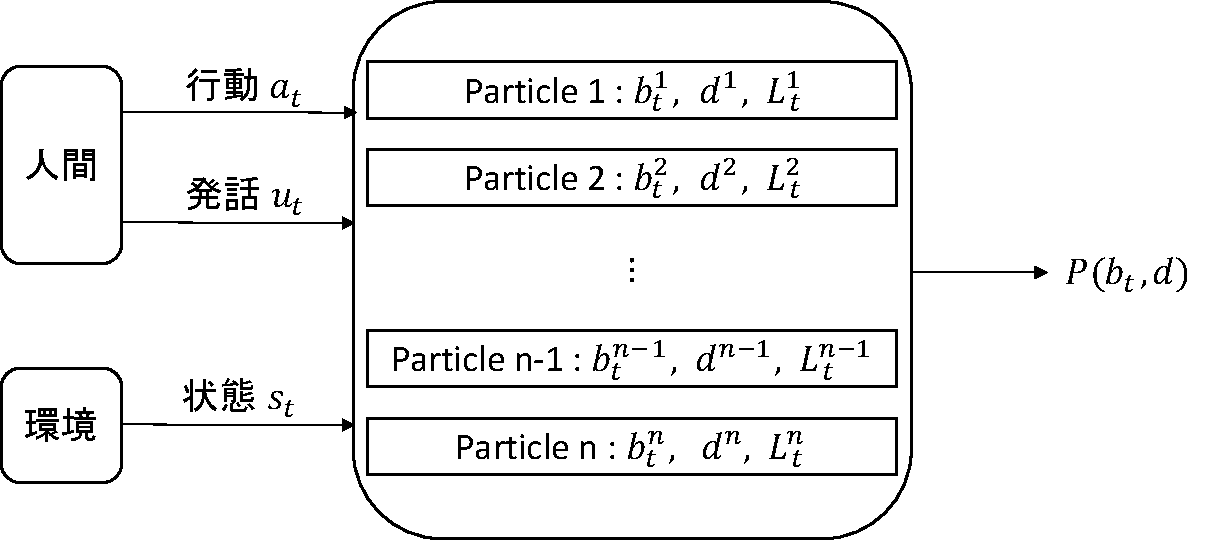
\includegraphics[scale=0.7]{./bt1.pdf}
    \caption{MIoM SCAINによる推定処理}
    \label{fig:sys_arc}
  \end{center}
\end{figure}
図\ref{fig:sys_arc}に示すように,MIoM SCAINは時刻$t$における人間の散策行動$a_t$,人間の発話文$u_t$および環境の状態$s_t$から信念と欲求の確率を出力する.MIoM SCAINは信念$b_t$と欲求$d$の組み合わせとその尤度$L_t$を持つパーティクルフィルタとして表現され,$a_t,u_t,s_t$とパーティクル$k$が持つ信念$b_t^k$と欲求$d^k$を基に尤度$L^k_t$が更新される.尤度$L^k_t$は式(\ref{pf})として表すことができる.
\begin{equation}
  \begin{split}
  \label{pf}
  L^k_t=P(b_t^k,d^k|s_{1:t},a_{1:t-1},u_{1:t-1})
  \end{split}
\end{equation}
ここで,$u_{1:t-1}$は,時刻$1$から時刻$t-1$までの人間の発話文履歴,$P(b_t,d|s_{1:t},a_{1:t-1},u_{1:t-1})$は,$s_{1:t},a_{1:t-1}およびu_{1:t-1}$から計算される信念$b_t$と欲求$d$の確率である.

\par
図\ref{fig:miom}にMIoM SCAINにおけるベイズ推定を表現するベイジアンネットワークを示す.$s_t$,$a_t$および$u_t$は観測値,$o_t$,$b_t$および$d$は確率変数として扱う.
\begin{figure}[htbp]
  \begin{center}
    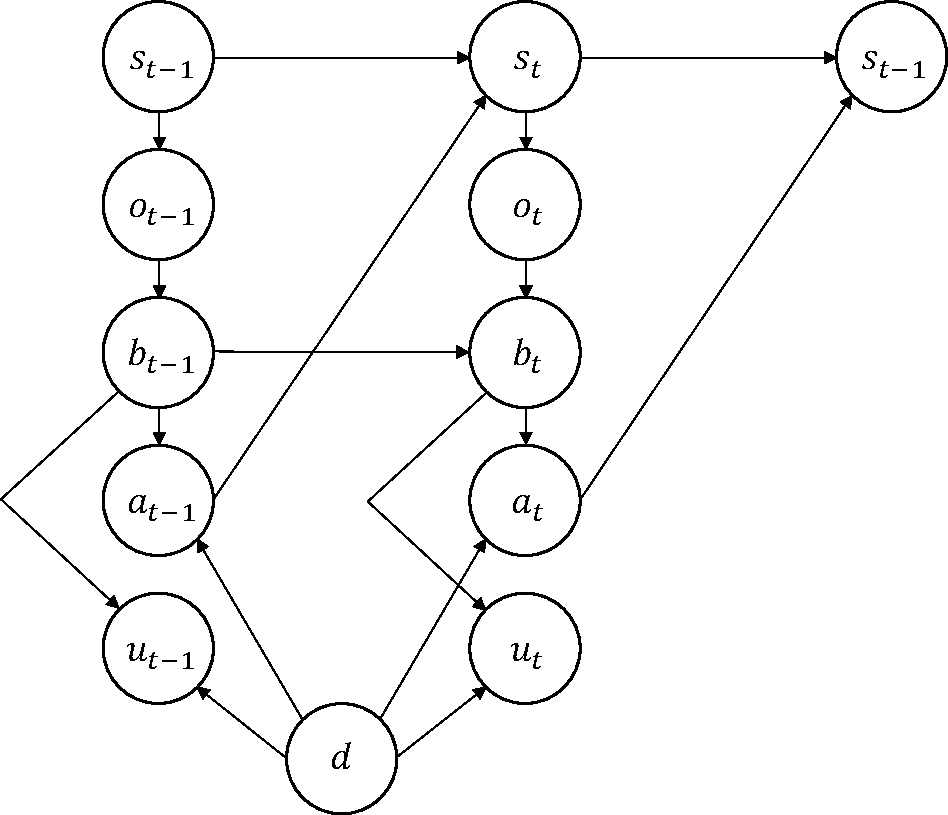
\includegraphics[scale=0.7]{./miom.pdf}
    \caption{MIoM SCAINにおけるベイズ推定を表現するベイジアンネットワーク}
    \label{fig:miom}
  \end{center}
\end{figure}
MIoM SCAINにおけるベイズ推定では,BToMと同様に時刻$t$における環境の状態$s_{t}$を基に人間の観測状況$o_{t}$が決まる.また$o_{t}$を基に人間の信念$b_{t}$が決まり,信念$b_{t}$と人間の欲求$d$から人間の散策行動$a_{t}$が決まる.それに加え,MIoM SCAINでは$b_t$と$d$から人間の発話文$u_t$が決まる.また散策行動$a_{t}$が起こることにより,環境の状態は$s_{t+1}$に変化し,人間の観測状況,信念,散策行動および人間の発話文が再び決定される.
% MIoM SCAINでは各パーティクルの尤度$L^k_t$を更新することを目的としている.
ベイズの定理と図\ref{fig:miom}における変数間の独立性より,式(\ref{eq_miom})が成り立つ.

\begin{equation}
  \begin{split}
  \label{eq_miom}
  L^k_t&=P(b_t^k,d^k|s_{1:t},a_{1:t-1},u_{1:t-1})\\
  &\propto P(b_t^k,d^k,s_{1:t},a_{1:t-1},u_{1:t-1})\\
  &= \sum_{b_{t-1}^k,o_t}P(b_t^k,d^k,s_{1:t},a_{1:t-1},u_{1:t-1},b_{t-1}^k,o_t)\\
  &= \sum_{b_{t-1}^k,o_t}P(b_t^k|d^k,s_{1:t},a_{1:t-1},u_{1:t-1},b_{t-1}^k,o_t)\cdot P(d^k,s_{1:t},a_{1:t-1},u_{1:t-1},b_{t-1}^k,o_t)\\
  &= \sum_{b_{t-1}^k,o_t}P(b_t^k|b_{t-1}^k,o_t)\cdot P(o_t|d^k,s_{1:t},a_{1:t-1},u_{1:t-1},b_{t-1}^k)\cdot P(d^k,s_{1:t},a_{1:t-1},u_{1:t-1},b_{t-1}^k)\\
  &= \sum_{b_{t-1}^k,o_t}P(b_t^k|b_{t-1}^k,o_t)\cdot P(o_t|s_t)\cdot P(s_t|s_{t-1},a_{t-1})\\
  &\hspace{3cm} \cdot P(a_{t-1}|b_{t-1}^k,d^k)\cdot P(u_{t-1}|b_{t-1}^k,d^k)\cdot P(b_{t-1}^k,d^k,s_{1:t-1},a_{1:t-2},u_{1:t-2})\\
  &\propto \sum_{b_{t-1}^k,o_t}P(b_t^k|b_{t-1}^k,o_t)\cdot P(o_t|s_t)\cdot P(s_t|s_{t-1},a_{t-1})\\
  &\hspace{3cm} \cdot P(a_{t-1}|b_{t-1}^k,d^k)\cdot P(u_{t-1}|b_{t-1}^k,d^k)\cdot P(b_{t-1}^k,d^k|s_{1:t-1},a_{1:t-2},u_{1:t-2})\\
  &= \sum_{b_{t-1}^k,o_t}P(b_t^k|b_{t-1}^k,o_t)\cdot P(o_t|s_t)\cdot P(s_t|s_{t-1},a_{t-1})\\
  &\hspace{3cm} \cdot P(a_{t-1}|b_{t-1}^k,d^k)\cdot P(u_{t-1}|b_{t-1}^k,d^k)\cdot L^k_{t-1}\\
  \end{split}
\end{equation}
ここで,$P(b_t^k|b_{t-1}^k,o_t)$は人間の観測状況$o_t$によってパーティクル$k$の信念$b_t^k$が更新される確率,$P(o_t|s_t)$は環境の状態$s_t$において人間が観測状況$o_t$を得る確率,$P(s_t|s_{t-1},a_{t-1})$は環境の状態$s_{t-1}$において人間が散策行動$a_{t-1}$を起こした時に環境の状態が$s_{t}$になる確率,$P(a_{t-1}|b_{t-1}^k,d^k)$はパーティクル$k$が信念$b_{t-1}^k$,欲求$d^k$を持つ時に散策行動$a_{t-1}$を起こす確率,$P(u_{t-1}|b_{t-1}^k,d^k)$はパーティクル$k$が信念$b_{t-1}^k$,欲求$d^k$を持っている時に人間が発話文$u_t$を発話する確率,$L_{t-1}^k$は時刻$t-1$におけるパーティクル$k$の尤度である.式(\ref{eq_miom})より,$L^k_t$は初期値$L^k_1$を決めて順次更新する計算により求めることができる.
% また,$L^k_t$は$P(b_t^k|b_{t-1}^k,o_t)$,$P(o_t|s_t)$,$P(s_t|s_{t-1},a_{t-1})$,$P(a_{t-1}|b_{t-1}^k,d^k)$および$(u_{t-1}|b_{t-1}^k,d^k)$の乗算として表すことができる.

\section{実装}
\par
% それぞれの生起確率がどのように計算されるかを記載
MIoM SCAINでは,式(\ref{eq_miom})により各パーティクルの尤度を逐次的に更新する.各パーティクルにおいて$P(b_t^k|b_{t-1}^k,o_t)\cdot P(o_t|s_t)$,$P(s_t|s_{t-1},a_{t-1})$,$P(a_{t-1}|b_{t-1}^k,d^k)$および$P(u_{t-1}|b_{t-1}^k,d^k)$をそれぞれ計算する.

\par
最初に,$P(b_t^k|b_{t-1}^k,o_t)\cdot P(o_t|s_t)$の計算方法について説明する.$P(b_t^k|b_{t-1}^k,o_t)\cdot P(o_t|s_t)$は,式(\ref{calc_b_o})により信念$b_t^k$と観測状況$o_t$を比較し計算する.
\begin{equation}
  \begin{split}
  \label{calc_b_o}
  P(b_t^k|b_{t-1}^k,o_t)\cdot P(o_t|s_t)=
  \begin{cases}
    1 & (b_t^kとo_tが一致する時) \\
    0 & (b_t^kとo_tが一致しない時)
  \end{cases}
  \end{split}
\end{equation}

\par
次に$P(s_t|s_{t-1},a_{t-1})$の計算方法について説明する.$P(s_t|s_{t-1},a_{t-1})$は,式(\ref{calc_s})により計算される.
\begin{equation}
  \begin{split}
  \label{calc_s}
  P(s_t|s_{t-1},a_{t-1})=
  \begin{cases}
    1 & (s_t=T(s_{t-1},a_{t-1})) \\
    0 & (otherwise)
  \end{cases}
  \end{split}
\end{equation}
ここで,関数$T(s_{t-1},a_{t-1})$は環境の状態$s_{t-1}$および散策行動$a_{t-1}$を入力とし,次の環境の状態$s_t$を出力する関数である.

\par
次に$P(a_{t-1}|b_{t-1}^k,d^k)$の計算方法について説明する.$P(a_{t-1}|b_{t-1}^k,d^k)$は式(\ref{calc_a})により計算される.
\begin{equation}
  \begin{split}
  \label{calc_a}
  P(a_{t-1}|b_{t-1}^k,d^k)=\mathrm{softmax}(Q_{t-1},\delta)
  \end{split}
\end{equation}
ここで,$Q_{t-1}$は散策行動$a_{t-1}$の予測報酬,$\delta$は$P(a_{t-1}|b_{t-1}^k,d^k)$への予測報酬$Q_{t-1}$の寄与を調整する定数である.

\par
最後に$P(u_{t-1}|b_{t-1}^k,d^k)$の計算方法について説明する.$P(u_{t-1}|b_{t-1}^k,d^k)$は,式(\ref{calc_u})により計算される.
\begin{equation}
  \begin{split}
  \label{calc_u}
  P(u_{t-1}|b_{t-1}^k,d^k)\propto \sum_{i=1}^n(\alpha+\beta_p)\cdot\mathrm{similarity}(u_{t-1},g_i)
  \end{split}
\end{equation}
ここで,$g_i$は信念$b_{t-1}^k$または欲求$d^k$になり得る環境中の対象物,関数$\mathrm{similarity}(u_{t-1},g_i)$は人間の発話文$u_{t-1}$および環境中の対象物$g_i$を入力とし,Word2Vec \cite{mikolov2013efficient}により人間の発話文$u_{t-1}$を分散表現に変換した後,信念$b_{t-1}^k$または欲求$d^k$になり得る環境中の対象物$g_i$との類似度を出力する関数,$\alpha$は環境中の対象物$g$が信念$b_{t-1}^k$にあたる場合において関数$\mathrm{similarity}(u_{t-1},g_i)$の出力の大きさを調整する定数,$\beta_p$は環境中の対象物$g_i$が欲求$d^k$の$p$番目に強い欲求にあたる場合において関数$\mathrm{similarity}(u_{t-1},g_i)$の出力の大きさを調整する定数,$n$は環境中に存在する対象物$g_i$の数を表す定数である.
